\documentclass{article}

\usepackage[margin=0.5in]{geometry}
\usepackage{multicol}
\usepackage{arcs}
\usepackage{tikz}

\title{Plane Geometry Set B}
\date{}
\author{}

\begin{document}
\maketitle
\noindent Problems should be solved without calculators unless otherwise specified.
Remember to explain how you solved a problem.
\begin{multicols}{2}
    \begin{enumerate}
        \item Points $A$, $B$, $Q$, $D$, and $C$ lie on the circle shown and the measures of arcs $\stackrel{\mbox{\large$\frown$}}{BQ}$ and $\stackrel{\mbox{\large$\frown$}}{QD}$ are $42^{\circ}$ and $38^{\circ}$ respectively.
            What is the sum of angles $P$ and $Q$?
            \begin{center}
                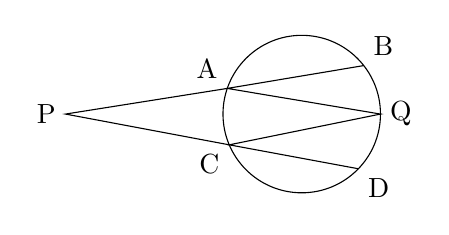
\begin{tikzpicture}
                    \draw (0,0) circle (1cm);
                    \foreach \name /\position /\angle /\radius in {A/{above left}/161/1, B/{above right}/38/1, C/{below left}/203/1, D/{below right}/316/1, P/{left}/180/3, Q/{right}/0/1}
                        \coordinate[label= \position:\name] (\name) at (\angle:\radius);
                    \draw (B) -- (A) -- (Q) -- (C) -- (D);
                    \draw (A) -- (P) -- (C);
                \end{tikzpicture}
            \end{center}
            \vspace{3cm}
        \item Kent draws a regular hexagon of side length $4$ cm and then draws a semicircle outward along each side.
            The total area enclosed by Kent's drawing can be expressed in simplest radical form, in terms of $\pi$, as $(a \cdot \sqrt{b} + c\pi)$.
            What is the value of $\frac{a}{b} + c$?
            \vspace{3cm}
        \item In the figure, if arc $\stackrel{\mbox{\large$\frown$}}{AB} = 60^{\circ}$ and arc $\stackrel{\mbox{\large$\frown$}}{DE} = 40^{\circ}$, then what is $\angle ACD$?
            \begin{center}
                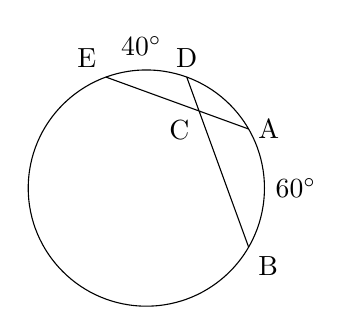
\begin{tikzpicture}
                    \draw (0,0) circle (1.5cm);
                    \coordinate[label=right:A] (A) at (30:1.5);
                    \coordinate[label=below right:B] (B) at (330:1.5);
                    \coordinate[label=above:D] (D) at (70:1.5);
                    \coordinate[label=above left:E] (E) at (110:1.5);
                    \draw (A) -- (E) (B) -- (D);
                    \coordinate[label=below left:C] (C) at (intersection of A--E and B--D);
                    \draw (92:1.8) node {$40^{\circ}$};
                    \draw (360:1.9) node {$60^{\circ}$};
                \end{tikzpicture}
            \end{center}
            \vspace{3cm}
        \item The incircle of a triangle is a circle tangent to all three sides of the triangle, as shown in this example.
            What is the radius of the incircle of a right triangle with side lengths of $12$, $35$ and $37$ mm?
            \begin{center}
                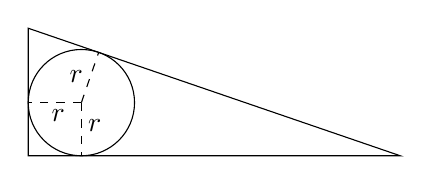
\begin{tikzpicture}
                    \draw (0,0) -- (0, 16.2mm) -- (47.25mm, 0) -- cycle;
                    \draw (6.75mm, 6.75mm) circle (6.75mm);
                    \begin{scope}[shift={(6.75mm,6.75mm)}]
                        \foreach \lineangle /\labelangle in {71/101,180/210,270/300}
                        {
                            \draw [dashed] (0,0) -- (\lineangle:6.75mm);
                            \draw (\labelangle:3.375mm) node {$r$};
                        }
                    \end{scope}
                \end{tikzpicture}
            \end{center}
            \vspace{3cm}
        \item Convex quadrilateral $WXYZ$ is inscribed in a circe.
            If m$\angle XYZ = 54^{\circ}$, what is the degree measure of $XWZ$?
            \vspace{3cm}
    \end{enumerate}
\end{multicols}
\end{document}